\documentclass[fleqn]{beamer}


\mode<presentation>
{
  \usetheme{default}
%   \useinnertheme[shadow=true]{rounded}

  \useinnertheme{circles}
  
%    \useoutertheme{infolines}
  % or ...
  \setbeamersize{text margin left=1em,text margin right=1em}

%   \setbeamercovered{transparent}
  % or whatever (possibly just delete it)

  \beamertemplatenavigationsymbolsempty
  
% Display frame numbers in footline
  \setbeamertemplate{footline}[frame number]

}

\usepackage{etex}
\usepackage[utf8]{inputenc}
\usepackage[T1]{fontenc}
\usepackage[english]{babel}
\usepackage{amsmath}
% \usepackage{amsthm}
\usepackage{stmaryrd}
\usepackage{lmodern}
\usepackage{mathpartir}

\usepackage[noend]{algpseudocode}





\usepackage{tikz}
% \usepackage{pgfplots}
% \pgfplotsset{compat=1.18}
% \usetikzlibrary{pgfplots.colorbrewer}
\usetikzlibrary{arrows,arrows.meta,positioning,calc,backgrounds}
\usetikzlibrary{overlay-beamer-styles}
\usetikzlibrary{shapes.geometric, decorations.pathreplacing}
\usetikzlibrary{shapes.callouts}
\usetikzlibrary{shapes.misc}
\usetikzlibrary{shapes.multipart}

\usetikzlibrary{fit}

\tikzset{
  -|-/.style={
    to path={
      (\tikztostart) -| ($(\tikztostart)!#1!(\tikztotarget)$) |- (\tikztotarget)
      \tikztonodes
    }
  },
  -|-/.default=0.5,
  |-|/.style={
    to path={
      (\tikztostart) |- ($(\tikztostart)!#1!(\tikztotarget)$) -| (\tikztotarget)
      \tikztonodes
    }
  },
  |-|/.default=0.5,
}

\tikzset{
  invisible/.style={opacity=0},
  visible on/.style={alt=#1{}{invisible}},
  alt/.code args={<#1>#2#3}{%
    \alt<#1>{\pgfkeysalso{#2}}{\pgfkeysalso{#3}} % \pgfkeysalso doesn't change the path
  },
}

% The goal is to translate
%    \overlaynode<red,blue>{hallo};
% into
%    \node[red]{hallo};
%    \node[blue]{hallo};
\makeatletter
\def\overlaynode<#1>#2;{
        \gdef\stacknodecommonpart{#2}
        \pgfkeys{/typeset node/.list={#1}}
        % we are lazy
        % pgfkeys will translate
        %    \pgfkeys{/typeset node/.list={red,blue}}
        % into
        %    \pgfkeys{/typeset node=red}
        %    \pgfkeys{/typeset node=blue}
}
\pgfkeys{
    /typeset node/.code={
        \edef\pgf@marshal{\noexpand\node[#1]\stacknodecommonpart;}
        \pgf@marshal
    }
}

\def\overlaynodedrawfill{\pgfutil@ifnextchar[{\overlaynodedrawfill@opt}{\overlaynodedrawfill@opt[]}}
\def\overlaynodedrawfill@opt[#1]<#2>#3;{
    \begin{scope}[transparency group,draw=black,fill=white,line cap=round,line join=round,#1]
        \pgfmathsetmacro\pgflinewidthdouble{2\pgflinewidth}
        \overlaynode<#2>[draw=pgfstrokecolor,line width=\pgflinewidthdouble]#3;
        \overlaynode<#2>[fill=pgffillcolor]#3;
    \end{scope}
}

\makeatother



\usepackage{listings}
\usepackage{lstautogobble}
\lstset{autogobble=true}

\usepackage{isasym}

\usepackage{cprotect}


\lstdefinelanguage{isabelle}{
  morekeywords={theorem,theorems,corollary,lemma,lemmas,locale,sublocale,global_interpretation,begin,end,fixes,assumes,shows,and,class,
    constrains , definition, defines, where, apply, done,unfolding, primrec, fun, using, by, for, uses, file,
    schematic_lemma, concrete_definition, prepare_code_thms, export_code, datatype, type_synonym, typedef, method,methods,
    proof, next, qed, show, have, hence, thus, interpretation, fix, context, sepref_definition,sepref_def,is,export_llvm,lift_definition,consts,specification
 } ,
  morekeywords=[2]{rec, return, bind, foreach, if, then, else, do, doN, let, in, res, spec, assert, assume, while, case, of,
    check,with_split,with_idxs,npar,nseq},
%  morekeywords=[3]{length,mod,insert},
%   morekeywords=[4]{simp,auto,intro,elim,rprems,refine_mono,refine_rcg},
  sensitive=True,
  morecomment=[s]{(\*}{\*)},
}


\lstdefinelanguage{Rust}{
    sensitive=true,
    morekeywords=[1]{
        as, break, const, continue, crate, else, enum, extern, false,
        fn, for, if, impl, in, let, loop, match, mod, move, mut, pub,
        ref, return, self, Self, static, struct, super, trait, true,
        type, unsafe, use, where, while, async, await, dyn
    },
    morekeywords=[2]{
        i8, i16, i32, i64, i128, isize,
        u8, u16, u32, u64, u128, usize,
        f32, f64, bool, char, str, String, Option, Result
    },
    morecomment=[l]{//},
    morecomment=[s]{/*}{*/},
    morestring=[b]",
    morestring=[b]'
}






\lstset{
    language=isabelle,
    mathescape=true,
    escapeinside={--"}{"},
    keywordstyle=\rm\bfseries,
    keywordstyle=[2]\rm\bfseries,
    keywordstyle=[3]\rm,
    keywordstyle=[4]\rm,
    showstringspaces=false,
    keepspaces=true,
    columns=[c]fullflexible}



% \lstset{numbers=left, numberstyle=\tiny, numbersep=5pt}

\newcommand*{\rc}[1]{\hfill\color{darkgray} --- #1}%

% \newcommand{\is}{\lstinline[language=isabelle,basicstyle=\normalsize\ttfamily\slshape]}
\newcommand{\is}{\lstinline[language=isabelle]}
\newcommand{\cs}{\lstinline[language=C++]}
\newcommand{\q}[1]{\mbox{\guilsinglleft{#1}\hspace{-.0pt}\guilsinglright}}
% \newcommand{\isai}[1]{\q{\lstinline[language=isabelle,basicstyle=\normalsize\ttfamily\slshape]{#1}}}
\cMakeRobust\q




\title{The Isabelle Refinement Framework}

% \subtitle
% {Subtitle} % (optional)

\author[Peter Lammich]{Peter Lammich}
% - Use the \inst{?} command only if the authors have different
%   affiliation.

\institute[UT] % (optional, but mostly needed)
{ University of Twente}
% - Use the \inst command only if there are several affiliations.
% - Keep it simple, no one is interested in your street address.

\date {November 2026 @ Groningen}
% {2008-12-01}


% If you have a file called "university-logo-filename.xxx", where xxx
% is a graphic format that can be processed by latex or pdflatex,
% resp., then you can add a logo as follows:

% \pgfdeclareimage[height=0.5cm]{university-logo}{university-logo-filename}
% \logo{\pgfuseimage{university-logo}}


% Delete this, if you do not want the table of contents to pop up at
% the beginning of each subsection:


% If you wish to uncover everything in a step-wise fashion, uncomment
% the following command: 

%\beamerdefaultoverlayspecification{<+->}



\begin{document}
% \input{macros}

\begin{frame}
  \titlepage
\end{frame}


\newcommand{\insertsectitle}{}


# Desirable Properties of Software
  \begin{center}
  \begin{tikzpicture}

    \node(center) at (0,0) {};

    \uncover<6->{
    \node(1)[circle, fill=green, minimum width = 3cm, anchor=center, opacity=.4] at ($(center.center)+(60:1.5cm)$) {};
    \node(2)[circle, fill=red, minimum width = 3cm, anchor=center, opacity=.4] at ($(center.center)+(180:1.5cm)$) {};
    \node(3)[circle, fill=blue, minimum width = 3cm, anchor=center, opacity=.4] at ($(center.center)+(300:1.5cm)$) {};
    \node at (center) {?};
    }

    \node<2-> at (1) {{\uncover<3->{Provably}} correct};
    \node<4-> at (2) {Fast};
    \node<5->[text width=2cm,align=center] at (3) {Manageable\\effort};


%     \draw (center.center)--(1.center);
%     \draw (center.center)--(2.center);
%     \draw (center.center)--(3.center);
  \end{tikzpicture}
  \end{center}

  \onslide<6->
  Choose two!

  \onslide<7->This Talk: making verifying fast software more manageable



\def\algoAugment{
  \begin{algorithmic}
    \Procedure{augment}{$g,f,p$}
      \State{$c_p \gets \min\{ g_f(u,v) \mid (u,v)\in p \}$}
      \ForAll{$(u,v)\in p$}
        \If{$(u,v)\in g$}~$f(u,v)\gets f(u,v) + c_p$
        \Else~$f(v,u)\gets f(v,u) - c_p$
        \EndIf
      \EndFor
      \Return{$f$}
    \EndProcedure
  \end{algorithmic}
}

\def\algoEdka{
  \begin{algorithmic}
    \Procedure{Edmonds-Karp}{$g,s,t$}
      \State{$f\gets \lambda(u,v).~0$}
      \While{exists augmenting path in $g_f$}
        \State{$p \gets {}$ shortest augmenting path}
        \State{$f \gets $\Call{augment}{$g,f,p$}}
      \EndWhile
    \EndProcedure
  \end{algorithmic}
}


#[t] Verifying Algorithms (e.g. Max-Flow)

  \begin{minipage}{.6\textwidth}
  \small\color{black}
%   \algoAugment
  \algoEdka
  \end{minipage}%
  \begin{minipage}{.39\textwidth}\hspace*{-2em}
    \hfill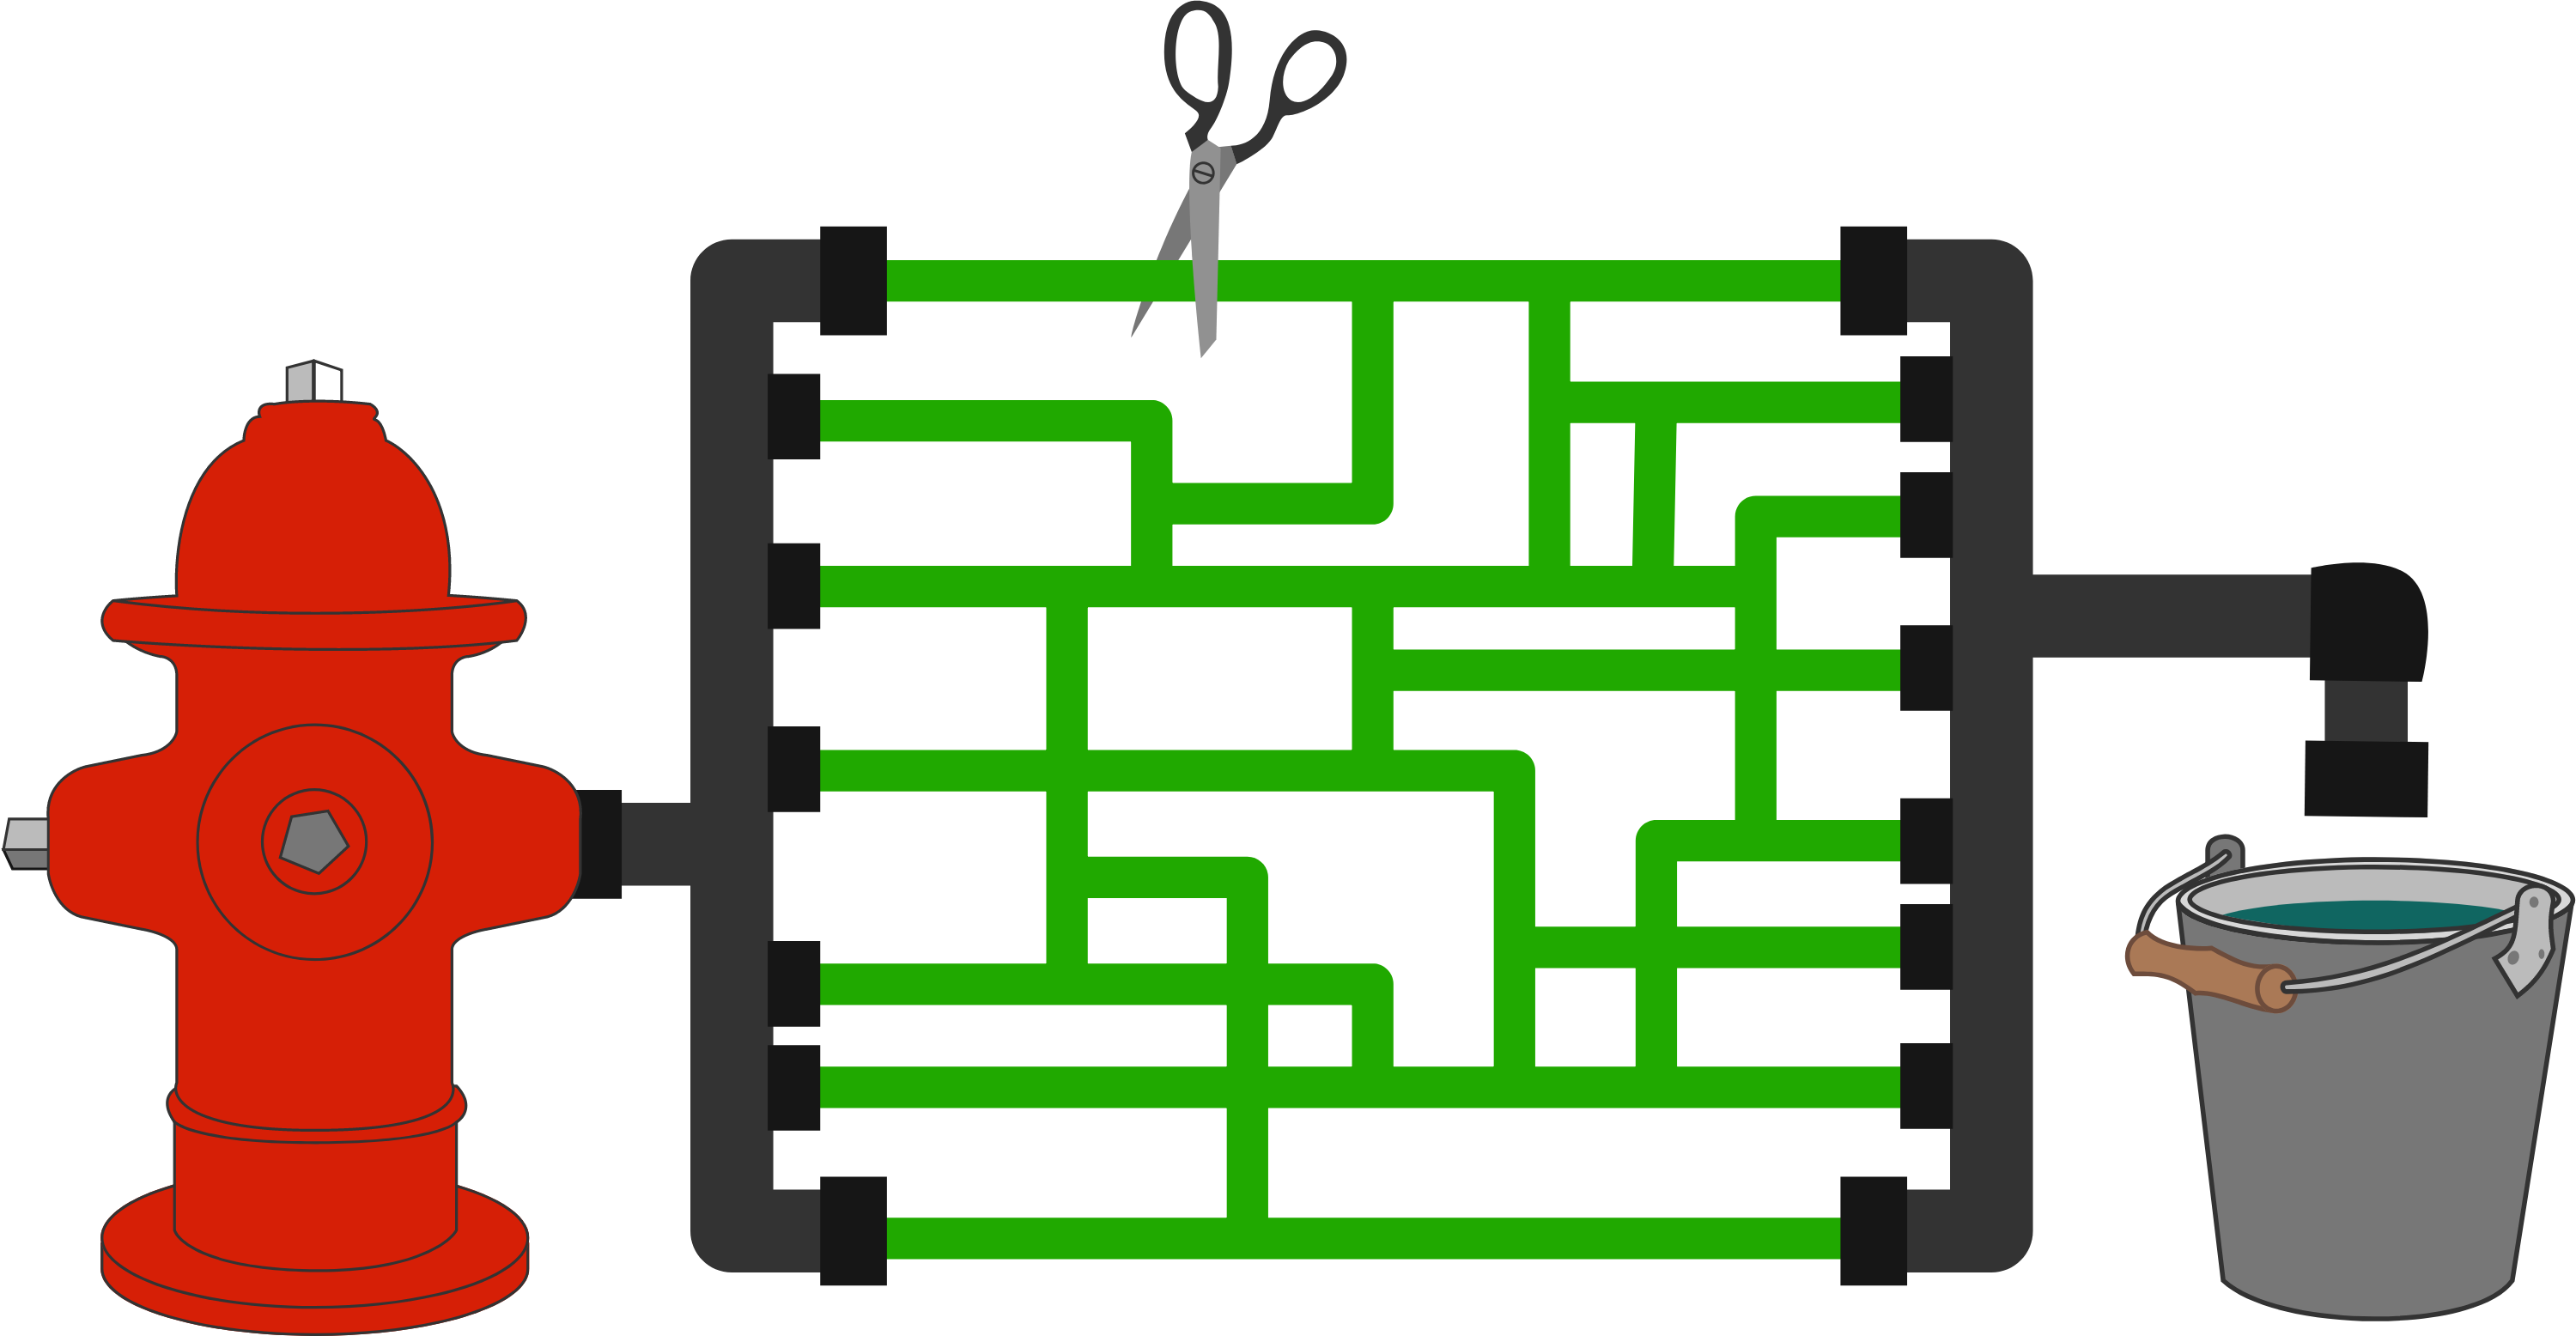
\includegraphics[width=\textwidth]{maxflow_mincut}
  \end{minipage}%

  \only<2-3>{
    \begin{theorem}[Ford-Fulkerson]
      For a flow network $g$ and flow $f$, the following 3 statements are equivalent
      \begin{enumerate}
        \item $f$ is a maximum flow
        \item the residual network $g_f$ contains no augmenting path
        \item $|f|$ is the capacity of a (minimal) cut of $g$
      \end{enumerate}
    \end{theorem}
    \uncover<3>{
      \begin{proof}
        a few pages of definitions and textbook proof (e.g. Cormen).

        using basic concepts such as numbers, sets, and graphs.
      \end{proof}
    }
  }

  \only<4-5>{
    \begin{theorem}[Termination in $O(VE)$ iterations]
      Let $\delta_f < |V|$ be the length of a shortest $s\textrm{--}t$ path in $g_f$.

      When augmenting with a shortest path,
      \begin{itemize}
        \item either $\delta_f$ increases
        \item or $\delta_f$ remains the same, and the number of edges in $g_f$ that lie on a shortest path decreases.
      \end{itemize}
    \end{theorem}
    \uncover<5>{
      \begin{proof}
        two more textbook pages.

        using lemmas about graphs and shortest paths.
      \end{proof}
    }
  }

  \only<6>{
    Still missing:
      * high-level optimizations
      * shortest path algorithm
      * data structures
      * low-level optimizations

  }

#! Implementation
  \begin{minipage}{.5\textwidth}
  \small
  \begin{lstlisting}[language=C++]
    int edmonds_karp(int s, int t) {
        int flow = 0;
        vector<int> parent(n);
        int new_flow;

        while (new_flow = bfs(s, t, parent)) {
            flow += new_flow;
            int cur = t;
            while (cur != s) {
                int prev = parent[cur];
                capacity[prev][cur] -= new_flow;
                capacity[cur][prev] += new_flow;
                cur = prev;
            }
        }

        return flow;
    }
  \end{lstlisting}
  \end{minipage}%
  \begin{minipage}{.39\textwidth}
    *: encoded concepts
    \begin{tikzpicture}
      \pause
      \node[rotate=30] at (0,1) {Ford-Fulkerson Theorem};
      \pause
      \node[rotate=70] at (.3,1.5) {Termination Argument};
      \pause
      \node[rotate=10] at (0,1) {Residual Network Optimization};
      \pause
      \node[rotate=0] at (1,1.5) {BFS Algorithm};
      \pause
      \node[rotate=45] at (0,2) {Graph Data Structure};
      \pause
      \node[rotate=80] at (-1,1.7) {Encoding Nodes as int};
      \node[rotate=20] at (-0.1,.7) {Arrays};
      \node[rotate=60] at (.4,1) {Queue data structure};


      \pause
      \node at (0,-2) {
\includegraphics[width=7cm]{proof_explosion}};

    \end{tikzpicture}

  \end{minipage}

# Stepwise Refinement
  \begin{tikzpicture}[auto]

    \tikzstyle{eannot}=[font=\small, align=left]

    \node[visible on=<2->] (fsp) {shortest-path-spec};
    \node[visible on=<3->] (bfs1) [below = of fsp] {bfs-1};
    \node[visible on=<5->] (bfs) [below = of bfs1] {bfs};

%     \draw [->] (fsp) -- node [label=right:{''textbook'' proof}] {} -- (bfs1);

    \draw[visible on=<3->,->] (fsp) to node[eannot,visible on=<4->] (l1) {''textbook'' proof} (bfs1);
    \draw[visible on=<5->,->] (bfs1) to node[eannot,visible on=<6->] (l2) {graph $\to$ adj.-list\\queue $\to$ ring-buffer} (bfs);

    \node[visible on=<7->,fit=(fsp)(bfs1)(bfs)(l1)(l2), shape=rectangle, draw] (boxbfs) {};

    \node[visible on=<8->] (cmf) [right = 3.5cm of fsp] {maxflow-spec};
    \node[visible on=<9->] (edka1) [below = of cmf] {edmonds\_karp-1};
    \node[visible on=<11->] (edka2) [below = of edka1] {edmonds\_karp-2};
    \node[visible on=<13->] (edka) [below = 2cm of edka2] {edmonds\_karp};

    \draw[visible on=<9->, ->] (cmf) to node[eannot,visible on=<10->] (l3) {''textbook'' proof} (edka1);
    \draw[visible on=<11->, ->] (edka1) to node[eannot,visible on=<12->] (l4) {residual graph optimization} (edka2);
    \draw[visible on=<13->, ->] (edka2) to node[eannot,visible on=<14->] (usebfs) {node $\to$ int\\graph $\to$ adj.-list\\capacity,flow $\to$ array\\shortest-path $\to$ bfs} (edka);

    \draw[visible on=<14->,->,dashed] (boxbfs) to[-|-] (usebfs.west);


    \only<15> {
    \overlaynodedrawfill[align=center]<
            {callout absolute pointer=(l1)},
            {callout absolute pointer=(l3)},
            {callout absolute pointer=(l4)}
        >
        [rectangle callout, below = of boxbfs, text width=4cm]
        {substantial ideas\\requires interactive proof}
    ;
    }

    \only<16> {
    \overlaynodedrawfill[align=center]<
            {callout absolute pointer=(l2)},
            {callout absolute pointer=(usebfs)}
        >
        [rectangle callout, below = of boxbfs, text width=4cm]
        {straightforward \\mainly automatic}
    ;
    }

  \end{tikzpicture}



# The Isabelle Refinement Framework (IRF)
  \definecolor{colA}{RGB}{11, 97,164}
  \definecolor{colB}{RGB}{204,246,  0}
  \definecolor{colC}{RGB}{166,  0,166}
  \definecolor{colD}{RGB}{255,146,  0}
  \definecolor{colTCB}{RGB}{255, 0, 0}

  Stepwise Refinement approach to verified algorithms in Isabelle/HOL


  \center
  \begin{tikzpicture}[node distance=.01\textwidth,outer sep=0pt,
  basicLayer/.style={
    draw=black,
    rounded corners,
    text width=.9\textwidth,
    font={\sffamily\bfseries\color{black}},
    align=center,
    minimum height=.03\textheight,
%    text height=12pt,
%    text depth=9pt
    },
  layerA/.style={basicLayer,fill=colA!30},
  layerB/.style={basicLayer,fill=colB!30},
  layerC/.style={basicLayer,fill=colC!30},
  layerD/.style={basicLayer,fill=colD!30},
  layerDD/.style={basicLayer,fill=colD!40,text width=.35\textwidth},
  layerTCB/.style={basicLayer,fill=colTCB!30,text width=.2\textwidth},
  layerTCBB/.style={basicLayer,fill=colTCB!40,text width=.4\textwidth},
  ]

  \node[layerA] (AlgDS) {Algorithms and Data Structures};

  \node[layerB, below=of AlgDS.south west, anchor=north west, text width=.437\textwidth] (ne) {Nres-Monad};
  \node[layerA, right=of ne.north east, anchor=north west, text width=.433\textwidth, minimum height=.134\textheight] (llDS) {Low-Level Algorithms \\and Data Structures};

  \node[layerB, below=of ne.south west, anchor=north west, text width=.437\textwidth] (sepref) {Sepref};

  \node[layerC, below=of sepref.south west, anchor=north west] (sepl) {Separation Logic and VCG};
  \node[layerD, below=of sepl.south west, anchor=north west, minimum height=.34\textheight] (sembox) {};

  \node[layerTCB, below left=of sembox.north east, minimum height=.32\textheight, text width=.46\textwidth] (tcbbox) {};


  \node[above right=of sembox.south west,font={\sffamily\bfseries\color{black}}] {Back End};

  \node[above left=of tcbbox.south east,font={\sffamily\bfseries\color{black}}] {Trusted Code Base};

%   \node[layerD, right=of sembox.west] (preproc) {Preprocessor};
%   \node[layerD, right=1cm of preproc] (instr) {Instructions};
%   \node[layerD, right=1cm of instr] (codegen) {Code Generator};

  \node[layerTCBB, below left=.3cm of tcbbox.north east] (codegen) {LLVM Code Generator};
%   \node[layerTCBB, left=1cm of codegen] (instr) {Instructions};
  \node[layerDD, left=1cm of codegen] (preproc) {LLVM Preprocessor};

  \node[layerTCBB, below =.5cm of codegen] (ihcodegen) {ImpHOL Code Generator};
%   \node[layerTCBB, left=1cm of codegen] (instr) {Instructions};
  \node[layerDD, left=1cm of ihcodegen] (ihpreproc) {ImpHOL Preprocessor};

%   \node[layerTCBB, below=of instr] (mmodel) {Memory Model};
%   \node[layerTCBB, below=of mmodel] (mmonad) {SNE-Monad};

  \draw[->] (preproc) -- (codegen);
  \draw[->] (ihpreproc) -- (ihcodegen);
%   \draw[->] (instr) -- (codegen);


  \end{tikzpicture}

% # Isabelle Refinement Framework
%   Software verification by stepwise refinement
%
%   * Based on Isabelle/HOL
%     * small TCB
%     * suited for complex background theory
%     * AFP: large library of reusable formalizations
%
%   * Down to LLVM-IR
%     * industrial strength IR
%     * easy integration with (unverified) components

#! The Nres-Monad
  Programs via nondeterminism-error monad
  {\small
  \begin{lstlisting}
    α nres  =  Fail  |  Spec (α ⇒ bool)

    return x        =  Spec (λr. r = x)

    bind Fail f     =  Fail
    bind (Spec P) f =  ⨆ { f x | P x }

    Spec P ≤ Spec Q  ⟷  ∀x. P x ⟶ Q x        m ≤ Fail
    ⨆S  =  if Fail ∈ S then Fail
           else Spec (λx. ∃P. Spec P ∈ S ∧ P x)
  \end{lstlisting}
  }

  * Refinement calculus with demonic ndet
  * Complete lattice (\is{⊥ = Spec (λ_. False)})
  * Bind is monotone, recursion ``for free'' via fixed points
  * Hoare triple: \is{P x ⟹ f x ≤ Spec (λr. Q r)}

#! Data Refinement
  Refinement relation \is{R} relates concrete and abstract type
    * e.g., \is$ls_rel ≡ { (xs,set xs) | xs. distinct xs }$

  Extension to nres: \is{⇓R m} all concrete results that refine an abstract result in \is{m}
  \begin{lstlisting}
    ⇓R Fail = Fail
    ⇓R (Spec P) = Spec (λc. ∃a. (c,a)∈R ∧ P a)
  \end{lstlisting}

  Refinement statement:
  \begin{lstlisting}
    ⟦(c⇩1,a⇩1)∈R⇩1; …; (c⇩n,a⇩n)∈R⇩n⟧ ⟹ f c⇩1 … c⇩n ≤ ⇓R (g a⇩1 … a⇩n)
  \end{lstlisting}
  * concise functor notation: \is{(f,g) ∈ R⇩1 → … → R⇩n → ⟨R⟩nres_rel}

  Examples:
  \begin{lstlisting}
    (ls_lookup, (∈)) ∈ Id → ls_rel → Id
    (ls_insert, Set.insert) ∈ Id → ls_rel → ls_rel
  \end{lstlisting}

#![t] Parametricity
  Used to handle nested data structures
  {\small
  \begin{lstlisting}
    ls_aux_rel ≡ { (xs,set xs) | xs. distinct xs }
    ⟨R⟩list_rel = { (cs,as). |cs|=|as| ∧ ∀i<|as|. (cs!i,as!i)∈R } --"\rc{natural relator}"

    ls_lookup eq x xs ≡ any (eq x) xs --"\rc{abstract over $=$}"

    (ls_lookup (=), (∈)) ∈ Id → ls_aux_rel → Id
    (ls_lookup, ls_lookup) ∈ (R→R→Id) → R → ⟨R⟩list_rel → Id --"\rc{free thm}"
  \end{lstlisting}
  \onslide<2->
  Combination yields: \\
    \is{(eq,(=))∈R→R→Id} \\ \is{⟹ (ls_lookup eq, (∈)) ∈ }
    \only<2>{\is{(R → ⟨R⟩list_rel → Id) O (Id → ls_aux_rel → Id)}}
    \only<3>{\is{R O Id → ⟨R⟩list_rel O ls_aux_rel → Id O Id}}
    \only<4->{\is{R → ⟨R⟩ls_rel → Id}}

  \onslide<4-> ~~~where \is{⟨R⟩ls_rel ≡ ⟨R⟩list_rel O ls_aux_rel}
  }

#! Automation
  * wp rules, e.g.
    \begin{lstlisting}
      P x ⟹ return x ≤ Spec P
      m ≤ Spec (λx. f x ≤ Spec Q) ⟹ bind m f ≤ Spec Q
    \end{lstlisting}

  * refinement rules, e.g.
    \begin{lstlisting}
      (return,return) ∈ R → ⟨R⟩nres_rel
      (bind,bind) ∈ ⟨R⇩1⟩nres_rel → (R⇩1→⟨R⇩2⟩nres_rel) → ⟨R⇩2⟩nres_rel
    \end{lstlisting}

  * Allows a syntax-driven VCG, and even synthesis of implementations.
  * Can be (partly) lifted to separation logic
    * VCG and synthesis for imperative programs
    * New challenges: ownership, closures


# Other Parts of the IRF
  * Sepref: synthesis of imperative code
    * from nres programs + data refinements to heap data structures
    * proves refinement w.r.t.\ separation logic
    * tools for composing data structures (parametricity)
  * Isabelle-LLVM back end
    * shallow embedding of LLVM fragment, separation logic + VCG
    * code export with C header for easy integration
    * parallel combinators, external functions with trusted specs % (malloc, fread, GMP)
    * dynamically checked assertions (e.g., out of memory, BigInt overflow)
  * Reusable libraries
    * data structures: arrays, dynamic arrays, bitsets, heaps, hash maps, \dots
    * algorithms: sorting, graph algorithms, \dots
    * fixed-width words, IEEE 754 floats with safe rounding

# Showcase: Bernoulli numbers
  \definecolor{verfill}{HTML}{E1F5EE}
  \definecolor{verdraw}{HTML}{0F6E56}
  \definecolor{trustfill}{HTML}{F1EFE8}
  \definecolor{trustdraw}{HTML}{5F5E5A}

  \tikzset{
    layer/.style={draw=verdraw, fill=verfill, rounded corners=3pt, thick,
      minimum width=12cm, minimum height=1.1cm, align=center},
    comp/.style={draw=verdraw!70, fill=white, rounded corners=2pt,
      minimum height=1cm, align=center, font=\small},
    trusted/.style={draw=trustdraw, fill=trustfill, dashed, thick},
    title/.style={font=\bfseries},
    sub/.style={font=\footnotesize},
  }
  \centering
  \resizebox{!}{0.75\textheight}{%
  \begin{tikzpicture}[node distance=3mm]

  % --- Number theory
  \node[layer] (nt) {%
    {\bfseries Number theory} {\footnotesize(Isabelle/HOL)}\\[-1pt]
    {\footnotesize Voronoi, Kummer, von Staudt--Clausen, bound on $|B_k|$}};

  % --- Efficient algorithms
  \node[comp, minimum width=2.15cm, above=5mm of nt.north west, anchor=south west,
        xshift=2mm] (mont) {Montgomery\\[-2pt]{\scriptsize modular mult.}};
  \node[comp, minimum width=2.15cm, right=2mm of mont] (crt)
    {Fast CRT\\[-2pt]{\scriptsize product tree}};
  \node[comp, minimum width=2.15cm, right=2mm of crt] (sieve)
    {Prime sieve\\[-2pt]{\scriptsize + factor map}};
  \node[comp, minimum width=2.15cm, right=2mm of sieve] (gen)
    {Generators\\[-2pt]{\scriptsize $g_p$, $\mathrm{ord}_p(2)$}};
  \node[comp, trusted, minimum width=2.15cm, right=2mm of gen] (gmp)
    {GMP\\[-2pt]{\scriptsize trusted spec}};
  \node[anchor=south, title] (eatitle) at ($(mont.north)!.5!(gmp.north)$)
    {Efficient algorithms {\normalfont\footnotesize(reusable)}};
  \begin{scope}[on background layer]
    \node[layer, fit=(mont)(gmp)(eatitle), inner sep=2mm, minimum width=12cm] (ea) {};
  \end{scope}

  % --- Harvey's core
  \node[layer, above=of ea] (core) {%
    {\bfseries Harvey's core: $N_k \bmod p$}\\[-1pt]
    {\footnotesize low-level tuned: blocking, tabulation, 32/64-bit select}};

  % --- Assembled algorithm
  \node[comp, minimum width=5.7cm, above=5mm of core.north west, anchor=south west,
        xshift=2mm] (par)
    {\bfseries Parallel {\normalfont(one machine)}\\[-2pt]
    {\scriptsize a-priori bound, sieve, parallel map, CRT}};
  \node[comp, minimum width=5.7cm, right=2mm of par] (dist)
    {\bfseries Distributed\\[-2pt]
    {\scriptsize workers on prime ranges, CRC32, CRT}};
  \node[anchor=south, title] (astitle) at ($(par.north)!.5!(dist.north)$)
    {Assembled algorithm};
  \begin{scope}[on background layer]
    \node[layer, fit=(par)(dist)(astitle), inner sep=2mm, minimum width=12cm] (as) {};
  \end{scope}

  % --- CLI
  \node[layer, trusted, above=of as] (cli) {%
    {\bfseries Thin CLI wrapper}\\[-1pt]
    {\footnotesize C++, unverified; calls exported LLVM functions}};

  % --- Legend
  \node[draw=verdraw, fill=verfill, thick, minimum width=5mm, minimum height=3mm,
        below=4mm of nt.south west, anchor=north west, xshift=2cm] (lv) {};
  \node[right=1mm of lv, sub] {verified (sepref down to LLVM)};
  \node[trusted, minimum width=5mm, minimum height=3mm,
        below=4mm of nt.south, anchor=north west, xshift=1.6cm] (lt) {};
  \node[right=1mm of lt, sub] {trusted / unverified};

  \end{tikzpicture}
  }
  \small

  * Competitive with Harvey's original implementation
  * Distributed: used to compute new record numbers $B_{10^{\lfloor8.5\rfloor}}$ and $B_{10^9}$
  * Randomized checker (no GMP): file encodes $B_k$, with proven error bound

# Showcase: UNSAT certificate checking

  \definecolor{verfill}{HTML}{E1F5EE}
  \definecolor{verdraw}{HTML}{0F6E56}
  \definecolor{trustfill}{HTML}{F1EFE8}
  \definecolor{trustdraw}{HTML}{5F5E5A}

  \tikzset{
    layer/.style={draw=verdraw, fill=verfill, rounded corners=3pt, thick,
      minimum width=12cm, minimum height=1.1cm, align=center},
    comp/.style={draw=verdraw!70, fill=white, rounded corners=2pt,
      minimum height=1cm, align=center, font=\small},
    trusted/.style={draw=trustdraw, fill=trustfill, dashed, thick},
    title/.style={font=\bfseries},
    sub/.style={font=\footnotesize},
  }

  \centering
  \resizebox{!}{0.75\textheight}{%
  \begin{tikzpicture}[node distance=3mm]

  % --- theory
  \node[layer] (nt) {%
    {\bfseries Specification \& theory} {\footnotesize(Isabelle/HOL)}\\[-1pt]
    {\footnotesize CNF semantics, DIMACS grammar ($\mathit{gM}$ monad), soundness of RUP checking}};

  % --- Efficient algorithms
  \node[comp, minimum width=2.15cm, above=5mm of nt.north west, anchor=south west,
        xshift=2mm] (mont) {Literals\\[-2pt]{\scriptsize u32, neg = \texttt{xor 1}}};
  \node[comp, minimum width=2.15cm, right=2mm of mont] (crt)
    {Clauses\\[-2pt]{\scriptsize 0-terminated}};
  \node[comp, minimum width=2.15cm, right=2mm of crt] (sieve)
    {Clause DB\\[-2pt]{\scriptsize pointer array}};
  \node[comp, minimum width=2.15cm, right=2mm of sieve] (gen)
    {Assignment\\[-2pt]{\scriptsize bits + set list}};
  \node[comp, trusted, minimum width=2.15cm, right=2mm of gen] (gmp)
    {\texttt{fread}\\[-2pt]{\scriptsize trusted spec}};
  \node[anchor=south, title] (eatitle) at ($(mont.north)!.5!(gmp.north)$)
    {Efficient data structures {\normalfont\footnotesize(with capacity bounds)}};
  \begin{scope}[on background layer]
    \node[layer, fit=(mont)(gmp)(eatitle), inner sep=2mm, minimum width=12cm] (ea) {};
  \end{scope}

  % --- core
  \node[layer, above=of ea] (core) {%
    {\bfseries Proof checker core: RUP steps}\\[-1pt]
    {\footnotesize unit-or-true checks along hints, clause builder, add/delete clauses}};

  % --- Assembled algorithm
  \node[comp, minimum width=5.7cm, above=5mm of core.north west, anchor=south west,
        xshift=2mm] (par)
    {\bfseries DIMACS parser\\[-2pt]
    {\normalfont\scriptsize verified against the grammar}};
  \node[comp, minimum width=5.7cm, right=2mm of par] (dist)
    {\bfseries Main checker loop\\[-2pt]
    {\normalfont\scriptsize LRAT parser on buffered certificate stream}};
  \node[anchor=south, title] (astitle) at ($(par.north)!.5!(dist.north)$)
    {Assembled checker {\normalfont\footnotesize(\texttt{read\_check\_lrat})}};
  \begin{scope}[on background layer]
    \node[layer, fit=(par)(dist)(astitle), inner sep=2mm, minimum width=12cm] (as) {};
  \end{scope}

  % --- CLI
  \node[layer, trusted, above=of as] (cli) {%
    {\bfseries Thin C wrapper}\\[-1pt]
    {\footnotesize unverified: command line, mmap formula, stream certificate from solver}};

  % --- Legend
  \node[draw=verdraw, fill=verfill, thick, minimum width=5mm, minimum height=3mm,
        below=4mm of nt.south west, anchor=north west, xshift=2cm] (lv) {};
  \node[right=1mm of lv, sub] {verified (sepref down to LLVM)};
  \node[trusted, minimum width=5mm, minimum height=3mm,
        below=4mm of nt.south, anchor=north west, xshift=1.6cm] (lt) {};
  \node[right=1mm of lt, sub] {trusted / unverified};

  \end{tikzpicture}
  }
  \small

  * on par with highly optimized, unverified lrat-trim
  * checks certificate while solver produces it
  * verified: accepts only if the .cnf file encodes an unsatisfiable formula

#! Showcase: Probabilistic Model Checking

  % Logo files: put them next to this .tex (any of .pdf/.png/.jpg).
  \newcommand{\dlogo}[2]{\IfFileExists{#1.pdf}{\includegraphics[height=#2]{#1.pdf}}{\IfFileExists{#1.png}{\includegraphics[height=#2]{#1.png}}{\IfFileExists{#1.jpg}{\includegraphics[height=#2]{#1.jpg}}{\fbox{\tiny #1}}}}}

  \definecolor{verfill}{HTML}{E1F5EE}
  \definecolor{verdraw}{HTML}{0F6E56}
  \definecolor{trustfill}{HTML}{F1EFE8}
  \definecolor{trustdraw}{HTML}{5F5E5A}
  \definecolor{gluefill}{HTML}{FAEEDA}
  \definecolor{gluedraw}{HTML}{854F0B}

  \tikzset{
    box/.style={rounded corners=2pt, thick, align=center, inner sep=4pt,
      minimum height=1.1cm, font=\small},
    ver/.style={box, draw=verdraw, fill=verfill},
    unv/.style={box, draw=trustdraw, fill=trustfill, dashed},
    glue/.style={box, draw=gluedraw, fill=gluefill, dashed, font=\scriptsize,
      minimum height=0.8cm},
    tool/.style={box, draw=trustdraw, fill=white, font=\scriptsize,
      minimum height=0.8cm},
    flow/.style={-{Stealth[length=2mm]}, thick, trustdraw},
    vflow/.style={-{Stealth[length=2mm]}, thick, verdraw},
    lbl/.style={font=\scriptsize, text=black!70},
    region/.style={rounded corners=4pt, draw=#1, thin, inner sep=6pt},
  }

  \hyphenpenalty=10000 \exhyphenpenalty=10000
  \centering
  \resizebox{!}{0.75\textheight}{%
  \begin{tikzpicture}

  % ================= Isabelle side (top) =================
  \node[ver, text width=3.6cm] (spec) at (0,8.6)
    {\textbf{Specification}\\[-1pt]{\scriptsize MDPs, reachability probabilities (Markov models library)}};
  \node[ver, text width=3.6cm] (ds) at (0,6.5)
    {\textbf{CSR MDP format}\\[-1pt]{\scriptsize formalised mcsta / UMB arrays, probabilities as $[\mathit{lb},\mathit{ub}]$ pairs}};
  \node[ver, text width=5.4cm] (alg) at (5.9,7.5)
    {\textbf{Verified pipeline}\\[-1pt]{\scriptsize SCC $\to$ MEC $\to$ min-/max-reduction $\to$ interval iteration with safe-rounding floats\\[1pt]
    one end-to-end theorem each for $P_{\min}$ and $P_{\max}$}};
  \node[ver, text width=2.4cm] (ll) at (11.6,7.5)
    {\textbf{LLVM IR}\\[-1pt]{\scriptsize + C header}};

  \draw[vflow] (spec.east) -- ++(0.5,0) |- ($(alg.west)+(0,0.2)$);
  \draw[vflow] (ds.east)   -- ++(0.5,0) |- ($(alg.west)+(0,-0.2)$);
  \draw[vflow] (alg) -- node[above,lbl]{\texttt{export\_llvm}} (ll);

  \begin{scope}[on background layer]
    \node[region=verdraw, fit=(spec)(ds)(alg)(ll), inner sep=8pt,
          label={[anchor=south west,font=\bfseries\small,text=verdraw]north west:Isabelle/HOL + Refinement Framework}] (isa) {};
  \end{scope}

  % library
  \node[tool, text width=4.0cm] (lib) at (8.0,4.6)
    {\textbf{Humble library}\\{\tiny compiled by Clang; full pipeline + individual algorithms}};
  \draw[flow] (isa.south -| ll) |- (lib.east);

  % ================= Humble tool (bottom left) =================
  \node[lbl] (umb) at (-2.4,1.2) {UMB file};
  \node[unv, text width=3.4cm] (wrap) at (0.9,1.2)
    {\textbf{C++ wrapper}\\[-1pt]{\scriptsize unpack, load JSON index, assemble arrays, round rationals to $[\mathit{lb},\mathit{ub}]$}};
  \node[ver, text width=2.2cm] (hp1) at (4.6,1.2)
    {\textbf{Humble}\\\textbf{pipeline}};
  \node[lbl, text width=1.8cm, align=center] (out1) at (4.6,-0.7) {bounds, reduced MDP};

  \draw[flow] (umb) -- (wrap);
  \draw[flow] (wrap) -- (hp1);
  \draw[flow] (hp1) -- (out1);

  \begin{scope}[on background layer]
    \node[region=trustdraw, fit=(wrap)(hp1)(out1), inner sep=8pt,
          label={[anchor=south west,font=\bfseries\small,text=trustdraw]north west:Humble tool (standalone)}] (tool) {};
  \end{scope}

  % ================= mcsta (bottom right) =================
  \node[unv, text width=2.6cm] (expl) at (9.6,1.2)
    {\textbf{Parsing \&}\\\textbf{exploration}\\[-1pt]{\scriptsize model $\to$ MDP arrays}};
  \node[ver, text width=2.2cm] (hp2) at (13.2,1.2)
    {\textbf{Humble}\\\textbf{pipeline}};
  \node[unv, text width=6.0cm] (rest) at (11.4,-0.9)
    {\textbf{Other analyses}\\[-1pt]{\scriptsize PTA, multi-objective, parameter spaces, POMDPs:\\[-2pt] unverified reductions to MDP reachability}};

  \draw[flow] (expl) -- (hp2);
  \draw[flow] (rest.north -| expl) -- node[left,lbl]{MDP} (expl.south);
  \draw[flow] (hp2.south) -- node[right,lbl]{bounds} (rest.north -| hp2);

  \begin{scope}[on background layer]
    \node[region=trustdraw, dashed, fit=(expl)(hp2)(rest), inner sep=8pt,
          label={[anchor=south west,font=\bfseries\small,text=trustdraw]north west:mcsta \dlogo{logo-modest}{0.6cm}}] (mc) {};
  \end{scope}

  % links from library
  \draw[vflow] (lib.south) -- ++(0,-0.6) -| node[pos=0.25,above,lbl]{static link} (hp1.north);
  \draw[vflow] (lib.south) -- ++(0,-0.6) -| node[pos=0.25,above,lbl]{C interface} (hp2.north);

  % ================= logos =================
  \node[anchor=north east, inner sep=4pt] at (isa.north east) {\dlogo{logo-isabelle}{0.9cm}};
%   \node[anchor=south east, inner sep=2pt] at (mc.north east)  {\dlogo{logo-modest}{0.6cm}};

  % ================= legend =================
  \node[ver, minimum height=0.35cm, minimum width=0.6cm, inner sep=0pt] (l1) at (-1.5,-2.6) {};
  \node[right=1mm of l1, lbl] (t1) {verified, correct by construction};
  \node[unv, minimum height=0.35cm, minimum width=0.6cm, inner sep=0pt, right=6mm of t1] (l2) {};
  \node[right=1mm of l2, lbl] (t2) {unverified};
  \node[tool, minimum height=0.35cm, minimum width=0.6cm, inner sep=0pt, right=6mm of t2] (l4) {};
  \node[right=1mm of l4, lbl] {trusted: Isabelle kernel, LLVM semantics, compiler, IEEE 754 hardware};

  \end{tikzpicture}
  }

  \small
  * within ~2× of Storm/mcsta, ~3× faster than Prism
  * found bugs in mcsta, Prism and Storm, in algorithms Humble verifies


# Conclusions
  Isabelle Refinement Framework

  * Refinement-based verification
    * scales to complex algorithms with competitive efficiency
    * small trusted base
    * integrates into existing systems via LLVM

  * Future work
    * bottom-up refinement (executable code first)
    * more concurrency (support wider class of algorithms)
    * partial verification in Isabelle-LLVM (exists for Imperative HOL)
    * AI-assisted proof engineering

  \vfill\pause

  \centering\emph{Verified software need not be slow!}



\end{document}






